\documentclass[10pt]{beamer}\usepackage[]{graphicx}\usepackage[]{color}
%% maxwidth is the original width if it is less than linewidth
%% otherwise use linewidth (to make sure the graphics do not exceed the margin)
\makeatletter
\def\maxwidth{ %
  \ifdim\Gin@nat@width>\linewidth
    \linewidth
  \else
    \Gin@nat@width
  \fi
}
\makeatother

\definecolor{fgcolor}{rgb}{0.345, 0.345, 0.345}
\newcommand{\hlnum}[1]{\textcolor[rgb]{0.686,0.059,0.569}{#1}}%
\newcommand{\hlstr}[1]{\textcolor[rgb]{0.192,0.494,0.8}{#1}}%
\newcommand{\hlcom}[1]{\textcolor[rgb]{0.678,0.584,0.686}{\textit{#1}}}%
\newcommand{\hlopt}[1]{\textcolor[rgb]{0,0,0}{#1}}%
\newcommand{\hlstd}[1]{\textcolor[rgb]{0.345,0.345,0.345}{#1}}%
\newcommand{\hlkwa}[1]{\textcolor[rgb]{0.161,0.373,0.58}{\textbf{#1}}}%
\newcommand{\hlkwb}[1]{\textcolor[rgb]{0.69,0.353,0.396}{#1}}%
\newcommand{\hlkwc}[1]{\textcolor[rgb]{0.333,0.667,0.333}{#1}}%
\newcommand{\hlkwd}[1]{\textcolor[rgb]{0.737,0.353,0.396}{\textbf{#1}}}%
\let\hlipl\hlkwb

\usepackage{framed}
\makeatletter
\newenvironment{kframe}{%
 \def\at@end@of@kframe{}%
 \ifinner\ifhmode%
  \def\at@end@of@kframe{\end{minipage}}%
  \begin{minipage}{\columnwidth}%
 \fi\fi%
 \def\FrameCommand##1{\hskip\@totalleftmargin \hskip-\fboxsep
 \colorbox{shadecolor}{##1}\hskip-\fboxsep
     % There is no \\@totalrightmargin, so:
     \hskip-\linewidth \hskip-\@totalleftmargin \hskip\columnwidth}%
 \MakeFramed {\advance\hsize-\width
   \@totalleftmargin\z@ \linewidth\hsize
   \@setminipage}}%
 {\par\unskip\endMakeFramed%
 \at@end@of@kframe}
\makeatother

\definecolor{shadecolor}{rgb}{.97, .97, .97}
\definecolor{messagecolor}{rgb}{0, 0, 0}
\definecolor{warningcolor}{rgb}{1, 0, 1}
\definecolor{errorcolor}{rgb}{1, 0, 0}
\newenvironment{knitrout}{}{} % an empty environment to be redefined in TeX

\usepackage{alltt}%
\usetheme{Boadilla}
\usecolortheme{seahorse}

\usepackage[utf8]{inputenc}%

% graphics
%% Figures %%%%%%%%%%%%%%%%%%%%%%%%%%%%%%%%%%%%%%%%%%%%%%%%%%
\usepackage{graphicx}
\usepackage{xcolor}%for color mixing

\usepackage{amsmath}%
\usepackage{amsfonts}%
\usepackage{amssymb}%
\usepackage{graphicx}

%%%%%%%%%%%%%%%%%%%%%%%%%%%%%%%%%%%%%%%%%%%%%%
%%%%%%%%%%%%%%%%% Doc info %%%%%%%%%%%%%%%%%%%
\title[\textbf{Intro to R}]{Introduction to R}
\date{\today}

%%%%%%%%%%%%%%%%%%%%%%%%%%%%%%%%%%%%%%%%%%%%%%
\IfFileExists{upquote.sty}{\usepackage{upquote}}{}
\begin{document}



\begin{frame}
\maketitle	
\end{frame}
%%%%%%%%%%%

\begin{frame}{R and RStudio}
  \begin{center}
    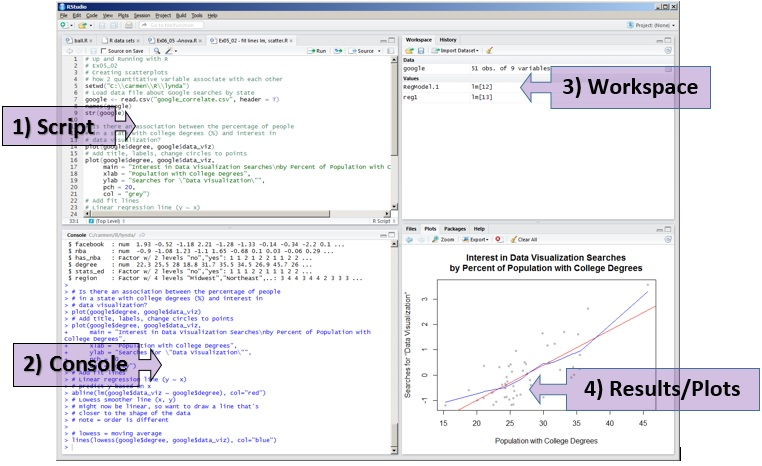
\includegraphics[width=0.8\textwidth]{Figures/rstudiolayout}
  \end{center}
\end{frame}
%%%%%%%%%%%

\begin{frame}{What R can do}

  \pause \begin{exampleblock}{Everything.$^{1,2}$}

  {\tiny $1$ Except think about your science}\\
  {\tiny $2$ Occasionally in a non efficient way}
  \end{exampleblock}

  \pause \begin{block}{What about RStudio?}
  \begin{itemize}
    \item Makes your life easier
    \item Many handy tricks
      \begin{itemize}
        \item Autocomplete suggestion
        \item Ctrl-Enter to send command to R
        \item str() and View() objects in Environment
        \item Files, packages, help selectors
        \item Version control\dots
      \end{itemize}
    \end{itemize}
  \end{block}
  
\end{frame}
%%%%%%%%%%%



\AtBeginSection[]
{
  \begin{frame}<beamer>
    \frametitle{}
    \tableofcontents[currentsection,hideothersubsections,subsectionstyle=hide]% down vote\tableofcontents[currentsection,currentsubsection,hideothersubsections,sectionstyle=show/hide,subsectionstyle=show/shaded/hide]
  \end{frame}
}

\section{About R-studio projects}

\begin{frame}{About R-studio projects}
Use them
\end{frame}
%%%%%%%%%%%%

\section{The mean}

\begin{frame}[fragile]{Calculating a mean: Arithmetic and assignment}

\begin{knitrout}
\definecolor{shadecolor}{rgb}{0.843, 0.867, 0.922}\color{fgcolor}\begin{kframe}
\begin{alltt}
  \hlstd{(}\hlnum{2} \hlopt{+} \hlnum{3} \hlopt{+} \hlnum{5} \hlopt{+} \hlnum{1}\hlstd{)} \hlopt{/} \hlnum{4}
\end{alltt}
\begin{verbatim}
[1] 2.75
\end{verbatim}
\end{kframe}
\end{knitrout}
\pause
\begin{knitrout}
\definecolor{shadecolor}{rgb}{0.843, 0.867, 0.922}\color{fgcolor}\begin{kframe}
\begin{alltt}
  \hlstd{a} \hlkwb{<-} \hlnum{2}
  \hlstd{b} \hlkwb{<-} \hlnum{3}
  \hlstd{c} \hlkwb{<-} \hlnum{5}
  \hlstd{d} \hlkwb{<-} \hlnum{1}

  \hlstd{(a} \hlopt{+} \hlstd{b} \hlopt{+} \hlstd{c} \hlopt{+} \hlstd{d)} \hlopt{/} \hlnum{4}
\end{alltt}
\begin{verbatim}
[1] 2.75
\end{verbatim}
\end{kframe}
\end{knitrout}
\pause
\begin{knitrout}
\definecolor{shadecolor}{rgb}{0.843, 0.867, 0.922}\color{fgcolor}\begin{kframe}
\begin{alltt}
  \hlstd{a} \hlkwb{<-} \hlnum{45}
  \hlstd{(a} \hlopt{+} \hlstd{b} \hlopt{+} \hlstd{c} \hlopt{+} \hlstd{d)} \hlopt{/} \hlnum{4}
\end{alltt}
\begin{verbatim}
[1] 13.5
\end{verbatim}
\end{kframe}
\end{knitrout}
\end{frame}
%%%%%%%%%%%

\begin{frame}[fragile]{Calculating a mean: using vectors}

\begin{knitrout}
\definecolor{shadecolor}{rgb}{0.843, 0.867, 0.922}\color{fgcolor}\begin{kframe}
\begin{alltt}
  \hlkwd{c}\hlstd{(}\hlnum{2}\hlstd{,}\hlnum{3}\hlstd{,}\hlnum{5}\hlstd{,}\hlnum{1}\hlstd{)} \hlcom{# c is for concatenate}
\end{alltt}
\begin{verbatim}
[1] 2 3 5 1
\end{verbatim}
\end{kframe}
\end{knitrout}
\pause
\begin{knitrout}
\definecolor{shadecolor}{rgb}{0.843, 0.867, 0.922}\color{fgcolor}\begin{kframe}
\begin{alltt}
 \hlstd{mydata} \hlkwb{<-} \hlkwd{c}\hlstd{(}\hlnum{2}\hlstd{,}\hlnum{3}\hlstd{,}\hlnum{5}\hlstd{,}\hlnum{1}\hlstd{)} \hlcom{# save the vector}
\end{alltt}
\end{kframe}
\end{knitrout}
\pause
\begin{knitrout}
\definecolor{shadecolor}{rgb}{0.843, 0.867, 0.922}\color{fgcolor}\begin{kframe}
\begin{alltt}
  mydata <- (2,3,5,1) \hlcom{# c is missing => error!}
\end{alltt}


{\ttfamily\noindent\bfseries\color{errorcolor}{Error: <text>:1:15: unexpected ','\\1:\ \  mydata <- (2,\\\ \ \ \ \ \ \ \ \ \ \ \ \ \ \ \ \ \ \textasciicircum{}}}\end{kframe}
\end{knitrout}
\end{frame}



%%%%%%%%%%%

  \begin{frame}[fragile]{Why bother with vectors?}
  Substitution:
\begin{knitrout}
\definecolor{shadecolor}{rgb}{0.843, 0.867, 0.922}\color{fgcolor}\begin{kframe}
\begin{alltt}
  \hlstd{mydata[}\hlnum{2}\hlstd{]} \hlkwb{<-} \hlnum{4}
  \hlstd{mydata}
\end{alltt}
\begin{verbatim}
[1] 2 4 5 1
\end{verbatim}
\end{kframe}
\end{knitrout}

  Vectorized operations:
\begin{knitrout}
\definecolor{shadecolor}{rgb}{0.843, 0.867, 0.922}\color{fgcolor}\begin{kframe}
\begin{alltt}
  \hlstd{mydata}\hlopt{*}\hlnum{5} \hlopt{+} \hlnum{2}
\end{alltt}
\begin{verbatim}
[1] 12 22 27  7
\end{verbatim}
\end{kframe}
\end{knitrout}
\end{frame}
%%%%%%%%%%%

\begin{frame}[fragile]{Exercise}

\begin{knitrout}
\definecolor{shadecolor}{rgb}{0.843, 0.867, 0.922}\color{fgcolor}\begin{kframe}
\begin{alltt}
  \hlopt{-}\hlnum{5}\hlopt{:}\hlnum{20}
\end{alltt}
\begin{verbatim}
 [1] -5 -4 -3 -2 -1  0  1  2  3  4  5  6  7  8  9 10 11 12 13 14 15 16 17
[24] 18 19 20
\end{verbatim}
\end{kframe}
\end{knitrout}

\end{frame}
%%%%%%%%%%%


\begin{frame}[fragile]{Calculating a mean: using functions}%shortcut

  How to use a function?
\begin{knitrout}
\definecolor{shadecolor}{rgb}{0.843, 0.867, 0.922}\color{fgcolor}\begin{kframe}
\begin{alltt}
  \hlopt{?}\hlstd{mean}
\end{alltt}
\end{kframe}
\end{knitrout}

  Or use \textbf{tab}
\pause

\begin{knitrout}
\definecolor{shadecolor}{rgb}{0.843, 0.867, 0.922}\color{fgcolor}\begin{kframe}
\begin{alltt}
\hlkwd{mean}\hlstd{(}\hlkwd{c}\hlstd{(}\hlnum{2}\hlstd{,}\hlnum{4}\hlstd{,}\hlnum{5}\hlstd{,}\hlnum{1}\hlstd{))}
\end{alltt}
\begin{verbatim}
[1] 3
\end{verbatim}
\begin{alltt}
\hlkwd{mean}\hlstd{(mydata)}
\end{alltt}
\begin{verbatim}
[1] 3
\end{verbatim}
\begin{alltt}
\hlkwd{mean}\hlstd{(}\hlkwc{x} \hlstd{= mydata)}
\end{alltt}
\begin{verbatim}
[1] 3
\end{verbatim}
\end{kframe}
\end{knitrout}


\end{frame}
%%%%%%%%%%

%%%%%%%%%%%%%%%%%%%%%%%%%%%%%%%%%%%%%%%%%%%%%%%%%%%%%%%%%%%%%%%%%%%%%%%%%%%%%%%%%
\section{Data-frames}

\begin{frame}[fragile]{Loading data}

\begin{knitrout}
\definecolor{shadecolor}{rgb}{0.843, 0.867, 0.922}\color{fgcolor}\begin{kframe}
\begin{alltt}
  \hlstd{trees} \hlkwb{<-} \hlkwd{read.csv}\hlstd{(}\hlstr{"trees.csv"}\hlstd{)}
\end{alltt}
\end{kframe}
\end{knitrout}
  \pause

\begin{knitrout}
\definecolor{shadecolor}{rgb}{0.843, 0.867, 0.922}\color{fgcolor}\begin{kframe}
\begin{alltt}
\hlkwd{str}\hlstd{(trees)}
\end{alltt}
\begin{verbatim}
'data.frame':	31 obs. of  3 variables:
 $ Girth : num  8.3 8.6 8.8 10.5 10.7 10.8 11 11 11.1 11.2 ...
 $ Height: int  70 65 63 72 81 83 66 75 80 75 ...
 $ Volume: num  10.3 10.3 10.2 16.4 18.8 19.7 15.6 18.2 22.6 19.9 ...
\end{verbatim}
\end{kframe}
\end{knitrout}

  Try also \texttt{summary}, \texttt{class}, \texttt{head}, \texttt{tail}
\end{frame}
%%%%%%%%%%%

\begin{frame}[fragile]{Access}

  \begin{block}{Bracket-syntax}
    \begin{itemize}
      \item Row: dataframe[row, ]
      \item Column: dataframe[ , column]
      \item Element: dataframe[row, column]
    \end{itemize}
  \end{block}

  \pause
\begin{knitrout}
\definecolor{shadecolor}{rgb}{0.843, 0.867, 0.922}\color{fgcolor}\begin{kframe}
\begin{alltt}
\hlstd{trees[,}\hlnum{1}\hlstd{]}
\hlstd{trees[}\hlnum{1}\hlopt{:}\hlnum{8}\hlstd{,]}
\hlstd{trees[}\hlkwd{c}\hlstd{(}\hlnum{2}\hlstd{,}\hlnum{1}\hlstd{,}\hlnum{2}\hlstd{),} \hlnum{3}\hlstd{]}
\hlstd{trees[,} \hlstr{"Height"}\hlstd{]}
\end{alltt}
\end{kframe}
\end{knitrout}

  \begin{block}{Dollar-syntax}
    \begin{itemize}
      \item Column \verb+ dataframe$column_name +
      \item Element \verb+ dataframe$column_name[row] +
    \end{itemize}
  \end{block}

\begin{knitrout}
\definecolor{shadecolor}{rgb}{0.843, 0.867, 0.922}\color{fgcolor}\begin{kframe}
\begin{alltt}
  \hlstd{trees}\hlopt{$}\hlstd{Height}
\end{alltt}
\end{kframe}
\end{knitrout}
\end{frame}
%%%%%%%%%%%

\begin{frame}{Time to think a tiny bit!}

  \textbf{Calculate the mean for all three variables in trees,\\ excluding the last (31st) record.}

\end{frame}
%%%%%%%%%%%

\begin{frame}[fragile]{Solution for one column}

  \textbf{Calculate the mean for all three variables in trees,\\ excluding the last (31st) record.}

\begin{knitrout}
\definecolor{shadecolor}{rgb}{0.843, 0.867, 0.922}\color{fgcolor}\begin{kframe}
\begin{alltt}
  \hlkwd{mean}\hlstd{(trees}\hlopt{$}\hlstd{Girth[}\hlnum{1}\hlopt{:}\hlnum{30}\hlstd{])}
  \hlkwd{mean}\hlstd{(trees[}\hlnum{1}\hlopt{:}\hlnum{30}\hlstd{,} \hlstr{"Girth"}\hlstd{])}
  \hlkwd{mean}\hlstd{(trees}\hlopt{$}\hlstd{Girth[}\hlopt{-}\hlnum{31}\hlstd{])}
  \hlkwd{mean}\hlstd{(trees[}\hlopt{-}\hlnum{31}\hlstd{,} \hlstr{"Girth"}\hlstd{])}
\end{alltt}
\end{kframe}
\end{knitrout}
\end{frame}
%%%%%%%%%%%
\begin{frame}[fragile]{How to get the row means?}
\begin{knitrout}
\definecolor{shadecolor}{rgb}{0.843, 0.867, 0.922}\color{fgcolor}\begin{kframe}
\begin{alltt}
\hlkwd{mean}\hlstd{(trees[}\hlnum{1}\hlstd{,])}
\hlkwd{mean}\hlstd{(trees[}\hlnum{2}\hlstd{,])}
\hlkwd{mean}\hlstd{(trees[...,])}
\end{alltt}
\end{kframe}
\end{knitrout}
  \pause
  \begin{center}:
    
\includegraphics[width=0.4\textwidth]{Figures/ineff}
  \end{center}
\end{frame}
%%%%%%%%%%%

\section{For-loop}

\begin{frame}[fragile]{How to get the row means? For-loops}

\begin{knitrout}
\definecolor{shadecolor}{rgb}{0.843, 0.867, 0.922}\color{fgcolor}\begin{kframe}
\begin{alltt}
  \hlkwd{for} (i in 1:N)
  \{
    something as a function of i
  \}\hlcom{#end of the loop}
\end{alltt}
\end{kframe}
\end{knitrout}

  \pause
\begin{knitrout}
\definecolor{shadecolor}{rgb}{0.843, 0.867, 0.922}\color{fgcolor}\begin{kframe}
\begin{alltt}
  \hlkwa{for} \hlstd{(i} \hlkwa{in} \hlnum{1}\hlopt{:}\hlnum{31}\hlstd{)}
  \hlstd{\{}
    \hlkwd{print}\hlstd{(i)}
  \hlstd{\}}
\end{alltt}
\end{kframe}
\end{knitrout}

\end{frame}
%%%%%%%%%%%

\begin{frame}[fragile]{How to get the row means? For-loops}

Start by buiding the code for 1 iteration (1 "i" value, e.g., 22):

\begin{knitrout}
\definecolor{shadecolor}{rgb}{0.843, 0.867, 0.922}\color{fgcolor}\begin{kframe}
\begin{alltt}
\hlkwd{mean}\hlstd{(}\hlkwd{as.numeric}\hlstd{(trees[}\hlnum{22}\hlstd{,]))}
\end{alltt}
\end{kframe}
\end{knitrout}

\pause 
We will want to store the result somewhere:
  
\begin{knitrout}
\definecolor{shadecolor}{rgb}{0.843, 0.867, 0.922}\color{fgcolor}\begin{kframe}
\begin{alltt}
  \hlstd{ResultMean} \hlkwb{<-} \hlkwd{vector}\hlstd{()} \hlcom{# we will store the results there}
  \hlstd{ResultMean[}\hlnum{22}\hlstd{]} \hlkwb{<-} \hlkwd{mean}\hlstd{(}\hlkwd{as.numeric}\hlstd{(trees[}\hlnum{22}\hlstd{,]))}
\end{alltt}
\end{kframe}
\end{knitrout}
  
  \pause
  
Now change 22 to "i" and write a loop around:
\begin{knitrout}
\definecolor{shadecolor}{rgb}{0.843, 0.867, 0.922}\color{fgcolor}\begin{kframe}
\begin{alltt}
\hlstd{ResultMean} \hlkwb{<-} \hlkwd{vector}\hlstd{()} \hlcom{# we will store the results there}
\hlkwa{for} \hlstd{(i} \hlkwa{in} \hlnum{1}\hlopt{:}\hlnum{31}\hlstd{)}
\hlstd{\{}
  \hlstd{ResultMean[i]} \hlkwb{<-} \hlkwd{mean}\hlstd{(}\hlkwd{as.numeric}\hlstd{(trees[i,]))}
\hlstd{\}}
\end{alltt}
\end{kframe}
\end{knitrout}

\end{frame}
%%%%%%%%%%%

\begin{frame}[fragile]{For-loops: your turn!}

Load rock data
\begin{knitrout}
\definecolor{shadecolor}{rgb}{0.843, 0.867, 0.922}\color{fgcolor}\begin{kframe}
\begin{alltt}
\hlstd{rock} \hlkwb{<-} \hlkwd{read.csv}\hlstd{(}\hlstr{"rock.csv"}\hlstd{)}
\end{alltt}
\end{kframe}
\end{knitrout}

  \centering
\textbf{\large Use a for loop to obtain column averages}

\end{frame}
%%%%%%%%%%%


\begin{frame}[fragile]{Solution}

Load rock data.
\begin{knitrout}
\definecolor{shadecolor}{rgb}{0.843, 0.867, 0.922}\color{fgcolor}\begin{kframe}
\begin{alltt}
\hlstd{rock} \hlkwb{<-} \hlkwd{read.csv}\hlstd{(}\hlstr{"rock.csv"}\hlstd{)}
\end{alltt}
\end{kframe}
\end{knitrout}

  \centering
\textbf{\large Use a for loop to obtain column averages}

\begin{knitrout}
\definecolor{shadecolor}{rgb}{0.843, 0.867, 0.922}\color{fgcolor}\begin{kframe}
\begin{alltt}
  \hlstd{storage} \hlkwb{<-} \hlkwd{vector}\hlstd{(}\hlkwc{length} \hlstd{=} \hlkwd{ncol}\hlstd{(rock))}
  \hlkwa{for} \hlstd{(i} \hlkwa{in} \hlnum{1}\hlopt{:}\hlkwd{ncol}\hlstd{(rock))}
  \hlstd{\{}
    \hlstd{storage[i]} \hlkwb{<-} \hlkwd{mean}\hlstd{(rock[,i])}
  \hlstd{\}}
\end{alltt}
\end{kframe}
\end{knitrout}
\end{frame}
%%%%%%%%%%%
\begin{frame}[fragile]{More concise alternative: apply functions}

\begin{knitrout}
\definecolor{shadecolor}{rgb}{0.843, 0.867, 0.922}\color{fgcolor}\begin{kframe}
\begin{alltt}
\hlkwd{apply}(X = dataframe, MARGIN = \hlkwd{1} (row) or \hlkwd{2} (col), FUN = function)
\end{alltt}
\end{kframe}
\end{knitrout}

  \pause

\begin{knitrout}
\definecolor{shadecolor}{rgb}{0.843, 0.867, 0.922}\color{fgcolor}\begin{kframe}
\begin{alltt}
\hlkwd{apply}\hlstd{(}\hlkwc{X} \hlstd{= rock,} \hlkwc{MARGIN} \hlstd{=} \hlnum{1}\hlstd{,} \hlkwc{FUN} \hlstd{= mean)}\hlcom{#by row (not meaningful)}
\hlkwd{apply}\hlstd{(}\hlkwc{X} \hlstd{= rock,} \hlkwc{MARGIN} \hlstd{=} \hlnum{2}\hlstd{,} \hlkwc{FUN} \hlstd{= mean)}\hlcom{#by column}
\end{alltt}
\end{kframe}
\end{knitrout}
\end{frame}
%%%%%%%%%%%
\begin{frame}[fragile]{Even better (worse)...}

\begin{knitrout}
\definecolor{shadecolor}{rgb}{0.843, 0.867, 0.922}\color{fgcolor}\begin{kframe}
\begin{alltt}
  \hlkwd{colMeans}\hlstd{(rock)}
  \hlkwd{rowMeans}\hlstd{(rock)}
\end{alltt}
\end{kframe}
\end{knitrout}

  \pause

  \begin{alertblock}{Trade-off concision  / flexibility}
    \begin{itemize}
      \item colMeans shortest, but does only means
      \item apply very flexible, but does only array/matrix/data-frame
      \item for-loop looks complex, but infinitely flexible
      \item (NB: your computer does a for-loop whether you see it or not)
    \end{itemize}
  \end{alertblock}

\end{frame}
%%%%%%%%%%%

\begin{frame}[fragile]{The last value}

Sometimes a function takes very long to run\\
\begin{knitrout}
\definecolor{shadecolor}{rgb}{0.843, 0.867, 0.922}\color{fgcolor}\begin{kframe}
\begin{alltt}
    \hlkwd{rowMeans}\hlstd{(rock[}\hlkwd{rep}\hlstd{(}\hlnum{1}\hlopt{:}\hlkwd{nrow}\hlstd{(rock),}\hlnum{100000}\hlstd{),])}
\end{alltt}
\end{kframe}
\end{knitrout}
\pause
What if you forgot to save the output to an object??

\pause 

\begin{knitrout}
\definecolor{shadecolor}{rgb}{0.843, 0.867, 0.922}\color{fgcolor}\begin{kframe}
\begin{alltt}
\hlstd{ourlasthope} \hlkwb{<-} \hlstd{.Last.value}
\end{alltt}
\end{kframe}
\end{knitrout}

\end{frame}


%%%%%%%%%%%%%%%%%%%%%%%%%%%%%%%%%%%%%%%%%%%%%%%%%%%%%%%%%%%%%%%%%%%%%%%%%%%%%%%%%

\section{While-loop}

\begin{frame}[fragile]{While-loop: idea}
Less common than for-loops\\
Stop the loop after a condition is met\\

\begin{knitrout}
\definecolor{shadecolor}{rgb}{0.843, 0.867, 0.922}\color{fgcolor}\begin{kframe}
\begin{alltt}
    \hlkwd{while}(condition TRUE)
    \{
      something
    \}
\end{alltt}
\end{kframe}
\end{knitrout}
  
\end{frame}
%%%%%%%%%%%

\begin{frame}[fragile]{What is the smallest reproductive rate necessary to obtain a growing population?}
\begin{knitrout}
\definecolor{shadecolor}{rgb}{0.843, 0.867, 0.922}\color{fgcolor}\begin{kframe}
\begin{alltt}
\hlkwd{library}\hlstd{(popbio)}
\hlstd{mat} \hlkwb{<-} \hlkwd{matrix}\hlstd{(}\hlkwd{c}\hlstd{(}\hlnum{0}\hlstd{,}\hlnum{0.8}\hlstd{,}\hlnum{1}\hlstd{,}\hlnum{0}\hlstd{),} \hlkwc{nrow} \hlstd{=} \hlnum{2}\hlstd{)}
\hlkwd{lambda}\hlstd{(mat)}
\end{alltt}
\begin{verbatim}
[1] 0.8944272
\end{verbatim}
\begin{alltt}
\hlstd{cond} \hlkwb{<-} \hlnum{1}
\hlkwa{while}\hlstd{(}\hlkwd{lambda}\hlstd{(mat)} \hlopt{<} \hlnum{1} \hlstd{)}
\hlstd{\{}
  \hlstd{mat[}\hlnum{1}\hlstd{,}\hlnum{2}\hlstd{]} \hlkwb{<-} \hlstd{mat[}\hlnum{1}\hlstd{,}\hlnum{2}\hlstd{]}\hlopt{+}\hlnum{0.001}
\hlstd{\}}
\hlstd{mat[}\hlnum{1}\hlstd{,}\hlnum{2}\hlstd{]}
\end{alltt}
\begin{verbatim}
[1] 1.251
\end{verbatim}
\end{kframe}
\end{knitrout}

\end{frame}
%%%%%%%%%%%

\begin{frame}[fragile]{But think twice before running a while loop\dots}
  
What happens if you run:
\begin{knitrout}
\definecolor{shadecolor}{rgb}{0.843, 0.867, 0.922}\color{fgcolor}\begin{kframe}
\begin{alltt}
\hlstd{x} \hlkwb{<-} \hlnum{1}
\hlkwa{while}\hlstd{(x}\hlopt{>}\hlnum{0}\hlstd{)}
\hlstd{\{}
  \hlstd{x} \hlkwb{<-} \hlstd{x} \hlopt{+} \hlnum{1}
\hlstd{\}}
\end{alltt}
\end{kframe}
\end{knitrout}

\end{frame}
%%%%%%%%%%%

\begin{frame}[fragile]{Looking for a rare event}

The function sample() takes 5 number between 1 and 6 (like 5 dice!):
\begin{knitrout}
\definecolor{shadecolor}{rgb}{0.843, 0.867, 0.922}\color{fgcolor}\begin{kframe}
\begin{alltt}
\hlstd{x} \hlkwb{<-} \hlkwd{sample}\hlstd{(}\hlkwc{x} \hlstd{=} \hlnum{1}\hlopt{:}\hlnum{6}\hlstd{,} \hlkwc{size} \hlstd{=} \hlnum{5}\hlstd{,} \hlkwc{replace} \hlstd{=} \hlnum{TRUE}\hlstd{)}
\end{alltt}
\end{kframe}
\end{knitrout}

Are all die equal?
\begin{knitrout}
\definecolor{shadecolor}{rgb}{0.843, 0.867, 0.922}\color{fgcolor}\begin{kframe}
\begin{alltt}
\hlkwd{all}\hlstd{(x} \hlopt{==} \hlstd{x[}\hlnum{1}\hlstd{])}
\end{alltt}
\begin{verbatim}
[1] FALSE
\end{verbatim}
\end{kframe}
\end{knitrout}

Are they ever going to be equal?
Write a while loop to find a case


\end{frame}
%%%%%%%%%%%%

\section{If-else statements}

\begin{frame}[fragile]{If-else statements}

\begin{knitrout}
\definecolor{shadecolor}{rgb}{0.843, 0.867, 0.922}\color{fgcolor}\begin{kframe}
\begin{alltt}
\hlkwd{if}(condition)
\{
  do something
\}
\end{alltt}
\end{kframe}
\end{knitrout}


\begin{knitrout}
\definecolor{shadecolor}{rgb}{0.843, 0.867, 0.922}\color{fgcolor}\begin{kframe}
\begin{alltt}
\hlkwd{if}(condition)
\{
  do something
\}else\{
  do something else
\}
\end{alltt}
\end{kframe}
\end{knitrout}

\end{frame}
%%%%%%%%%%%%

\begin{frame}[fragile]{If-else statements}

For instance:
\begin{knitrout}
\definecolor{shadecolor}{rgb}{0.843, 0.867, 0.922}\color{fgcolor}\begin{kframe}
\begin{alltt}
\hlkwa{for} \hlstd{(i} \hlkwa{in} \hlnum{1}\hlopt{:}\hlnum{10}\hlstd{)}
\hlstd{\{}
  \hlkwa{if}\hlstd{(i} \hlopt{<} \hlnum{6}\hlstd{)}
  \hlstd{\{}
    \hlkwd{print}\hlstd{(}\hlstr{"tofu"}\hlstd{)}
  \hlstd{\}}\hlkwa{else}\hlstd{\{}
    \hlkwd{print}\hlstd{(}\hlstr{"bacon"}\hlstd{)}
  \hlstd{\}}
\hlstd{\}}
\end{alltt}
\end{kframe}
\end{knitrout}
\end{frame}
%%%%%%%%%%%


\section{Visualisation}

\begin{frame}[fragile]{plot function}

\begin{knitrout}
\definecolor{shadecolor}{rgb}{0.843, 0.867, 0.922}\color{fgcolor}\begin{kframe}
\begin{alltt}
\hlkwd{plot}\hlstd{(rock)}
\end{alltt}
\end{kframe}
\includegraphics[width=0.8\textwidth,height=0.6\textwidth]{figure/plorock-1} 

\end{knitrout}

\end{frame}
%%%%%%%%%%%

\begin{frame}[fragile]{plot function}

\begin{knitrout}
\definecolor{shadecolor}{rgb}{0.843, 0.867, 0.922}\color{fgcolor}\begin{kframe}
\begin{alltt}
\hlkwd{plot}\hlstd{(rock}\hlopt{$}\hlstd{peri)}
\end{alltt}
\end{kframe}
\includegraphics[width=0.8\textwidth,height=0.6\textwidth]{figure/plorock2-1} 

\end{knitrout}

\end{frame}
%%%%%%%%%%%

\begin{frame}[fragile]{plot function}

\begin{knitrout}
\definecolor{shadecolor}{rgb}{0.843, 0.867, 0.922}\color{fgcolor}\begin{kframe}
\begin{alltt}
\hlkwd{plot}\hlstd{(}\hlkwc{x} \hlstd{= rock}\hlopt{$}\hlstd{peri,} \hlkwc{y} \hlstd{= rock}\hlopt{$}\hlstd{area)}
\end{alltt}
\end{kframe}
\includegraphics[width=0.8\textwidth,height=0.6\textwidth]{figure/plorock3-1} 

\end{knitrout}

\end{frame}
%%%%%%%%%%%

\begin{frame}[fragile]{plot function}

\begin{knitrout}
\definecolor{shadecolor}{rgb}{0.843, 0.867, 0.922}\color{fgcolor}\begin{kframe}
\begin{alltt}
\hlkwd{plot}\hlstd{(}\hlkwc{x} \hlstd{= rock}\hlopt{$}\hlstd{peri,} \hlkwc{y} \hlstd{= rock}\hlopt{$}\hlstd{area,} \hlkwc{main} \hlstd{=} \hlstr{"Eureka!"}\hlstd{,}
     \hlkwc{xlab} \hlstd{=} \hlstr{"Perimeter"}\hlstd{,} \hlkwc{ylab} \hlstd{=} \hlstr{"area"}\hlstd{,} \hlkwc{col}\hlstd{=}\hlstr{"blue"}\hlstd{,} \hlkwc{pch}\hlstd{=}\hlnum{2}\hlstd{)}
\end{alltt}
\end{kframe}
\includegraphics[width=0.8\textwidth,height=0.6\textwidth]{figure/plorock4-1} 

\end{knitrout}
\end{frame}
%%%%%%%%%%%

\begin{frame}[fragile]{plot function: back to the mean}
\begin{knitrout}
\definecolor{shadecolor}{rgb}{0.843, 0.867, 0.922}\color{fgcolor}\begin{kframe}
\begin{alltt}
\hlkwd{data}\hlstd{(}\hlstr{"iris"}\hlstd{)}
\end{alltt}
\end{kframe}
\end{knitrout}
\end{frame}
%%%%%%%%%%%

\begin{frame}[fragile]{plot function: back to the mean}
\begin{knitrout}
\definecolor{shadecolor}{rgb}{0.843, 0.867, 0.922}\color{fgcolor}\begin{kframe}
\begin{alltt}
\hlkwd{plot}\hlstd{(iris}\hlopt{$}\hlstd{Sepal.Length,} \hlkwc{col}\hlstd{=iris}\hlopt{$}\hlstd{Species)}
\end{alltt}
\end{kframe}
\includegraphics[width=0.8\textwidth,height=0.6\textwidth]{figure/iris1-1} 

\end{knitrout}
\end{frame}
%%%%%%%%%%%

\begin{frame}[fragile]{boxplots}
\begin{knitrout}
\definecolor{shadecolor}{rgb}{0.843, 0.867, 0.922}\color{fgcolor}\begin{kframe}
\begin{alltt}
\hlkwd{boxplot}\hlstd{(iris}\hlopt{$}\hlstd{Sepal.Length} \hlopt{~} \hlstd{iris}\hlopt{$}\hlstd{Species)}
\end{alltt}
\end{kframe}
\includegraphics[width=0.8\textwidth,height=0.6\textwidth]{figure/plorock5-1} 
\begin{kframe}\begin{alltt}
\hlcom{#or plot(iris$Sepal.Length ~ iris$Species)}
\end{alltt}
\end{kframe}
\end{knitrout}

\end{frame}
%%%%%%%%%%%
%%%%%%%%%%%%%%%%%%%%%%%%%%%%%%%%%%%%%%%%%%%%%%%%%%%%%%%%%%%%%%%%%%%%%%%%%%%%%%%%%
\section{T-test}

\begin{frame}[fragile]{Student's T.test introduction}% presenting the test, the output...
\begin{knitrout}
\definecolor{shadecolor}{rgb}{0.843, 0.867, 0.922}\color{fgcolor}\begin{kframe}
\begin{alltt}
\hlopt{?}\hlstd{t.test}
\end{alltt}
\end{kframe}
\end{knitrout}

  \pause
\begin{knitrout}
\definecolor{shadecolor}{rgb}{0.843, 0.867, 0.922}\color{fgcolor}\begin{kframe}
\begin{alltt}
\hlkwd{t.test}\hlstd{(}\hlnum{1}\hlopt{:}\hlnum{10}\hlstd{,} \hlkwc{y} \hlstd{=} \hlkwd{c}\hlstd{(}\hlnum{7}\hlopt{:}\hlnum{20}\hlstd{))}
\end{alltt}
\begin{verbatim}

	Welch Two Sample t-test

data:  1:10 and c(7:20)
t = -5.4349, df = 21.982, p-value = 1.855e-05
alternative hypothesis: true difference in means is not equal to 0
95 percent confidence interval:
 -11.052802  -4.947198
sample estimates:
mean of x mean of y 
      5.5      13.5 
\end{verbatim}
\end{kframe}
\end{knitrout}

\end{frame}
%%%%%%%%%%%

\begin{frame}[fragile]{T.test introduction}% presenting the test, the output...

\begin{knitrout}
\definecolor{shadecolor}{rgb}{0.843, 0.867, 0.922}\color{fgcolor}\begin{kframe}
\begin{alltt}
  \hlkwd{boxplot}\hlstd{(}\hlkwd{c}\hlstd{(}\hlnum{1}\hlopt{:}\hlnum{10}\hlstd{,} \hlnum{7}\hlopt{:}\hlnum{20}\hlstd{)} \hlopt{~} \hlkwd{c}\hlstd{(}\hlkwd{rep}\hlstd{(}\hlnum{1}\hlstd{,}\hlnum{10}\hlstd{),} \hlkwd{rep}\hlstd{(}\hlnum{2}\hlstd{,} \hlnum{14}\hlstd{)))}
\end{alltt}
\end{kframe}
\includegraphics[width=0.8\textwidth,height=0.6\textwidth]{figure/unnamed-chunk-43-1} 

\end{knitrout}
\end{frame}
%%%%%%%%%%%

\begin{frame}[fragile]{Are irises different?}

  \textbf{Use t-tests to compare species in the iris dataset}

  \begin{center}
    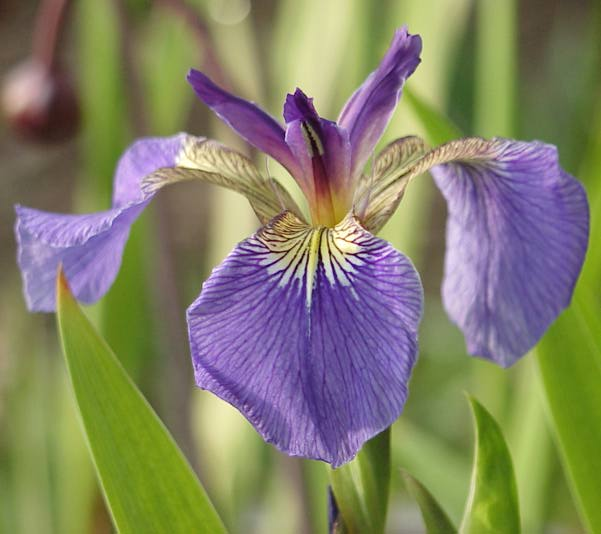
\includegraphics[height=0.6\textwidth]{Figures/iris}
  \end{center}
\end{frame}
%%%%%%%%%%%

\begin{frame}[fragile]{Are irises different? Solution}

  \textbf{Use t-tests to compare species in the iris dataset}

  Sorry, I was mean and forgot to tell about subsetting, which you needed here.\\
  Subset to the species \textit{setosa}:
\begin{knitrout}
\definecolor{shadecolor}{rgb}{0.843, 0.867, 0.922}\color{fgcolor}\begin{kframe}
\begin{alltt}
  \hlstd{iris[iris}\hlopt{$}\hlstd{Species} \hlopt{==} \hlstr{"setosa"}\hlstd{, ]}
\end{alltt}
\end{kframe}
\end{knitrout}

  One t-test for sepal length between \textit{setosa} and \textit{versicolor}:
\begin{knitrout}
\definecolor{shadecolor}{rgb}{0.843, 0.867, 0.922}\color{fgcolor}\begin{kframe}
\begin{alltt}
  \hlkwd{t.test}\hlstd{(}\hlkwc{x} \hlstd{= iris}\hlopt{$}\hlstd{Sepal.Length[iris}\hlopt{$}\hlstd{Species} \hlopt{==} \hlstr{"setosa"}\hlstd{],}
        \hlkwc{y} \hlstd{= iris}\hlopt{$}\hlstd{Sepal.Length[iris}\hlopt{$}\hlstd{Species} \hlopt{==} \hlstr{"versicolor"}\hlstd{])}
\end{alltt}
\end{kframe}
\end{knitrout}


\end{frame}
%%%%%%%%%%%

\end{document}
